%Formatação de Textos Longos
\documentclass[a4paper, 12pt]{article}
\usepackage[top=2cm, bottom=2cm, left=2.5cm, right=2.5cm]{geometry}
\usepackage[utf8]{inputenc}
\usepackage{amsmath, amsfonts, amssymb} 
\usepackage{graphicx}
\usepackage{float} 
\usepackage[brazil]{babel} %colocou "brazil" em vez de "portuguese" para que o título do sumário esteja escrito como "Sumário", e não como "Conteúdo", como tinha sido escrito
\usepackage{indentfirst} %coloca parágrafo na primeira linha de um texto após colocar uma seção

%comandos para fazer o título
\title{Aqui vem o título do trabalho.}
\author{Nome do Autor \\ email@domínio.com.br}
\date{2018} %se você deixar as chaves em branco, o programa irá retirar a data
        %se você retirar o comando em si (\date{}), o programa irá colocar a data da última vez que você compilou o arquivo
        %se você colocar uma data entre as chaves, o documento apresentará uma data fixa

\begin{document}

\maketitle %comando para pegar os dados do título (preâmbulo) e exibí-los

\tableofcontents %inserir sumário

\newpage % pula uma página

\listoffigures %colocar lista de figuras

\newpage

\listoftables %inserir lista de tabelas

\newpage

%se você está em um artigo, você pode dividir o documento em seções. E dessas seções, pode-se dividí-lo em subseções (e as subseções em subsubseções) 

\section{Introdução} %cria uma parte (seção) no documento

Aqui vem o texto. Aqui vem o texto. Aqui vem o texto. Aqui vem o texto. 
Aqui vem o texto. Aqui vem o texto. Aqui vem o texto. Aqui vem o texto. 
Aqui vem o texto. Aqui vem o texto. Aqui vem o texto. Aqui vem o texto. 
Aqui vem o texto. Aqui vem o texto. Aqui vem o texto. Aqui vem o texto. 
Aqui vem o texto. Aqui vem o texto. Aqui vem o texto. Aqui vem o texto.  \cite{meuatalho} %citação de referência blbiográfica (definida no arquivo 2018-11-27_referencia.bib)

\begin{figure}[htb]
    \centering
    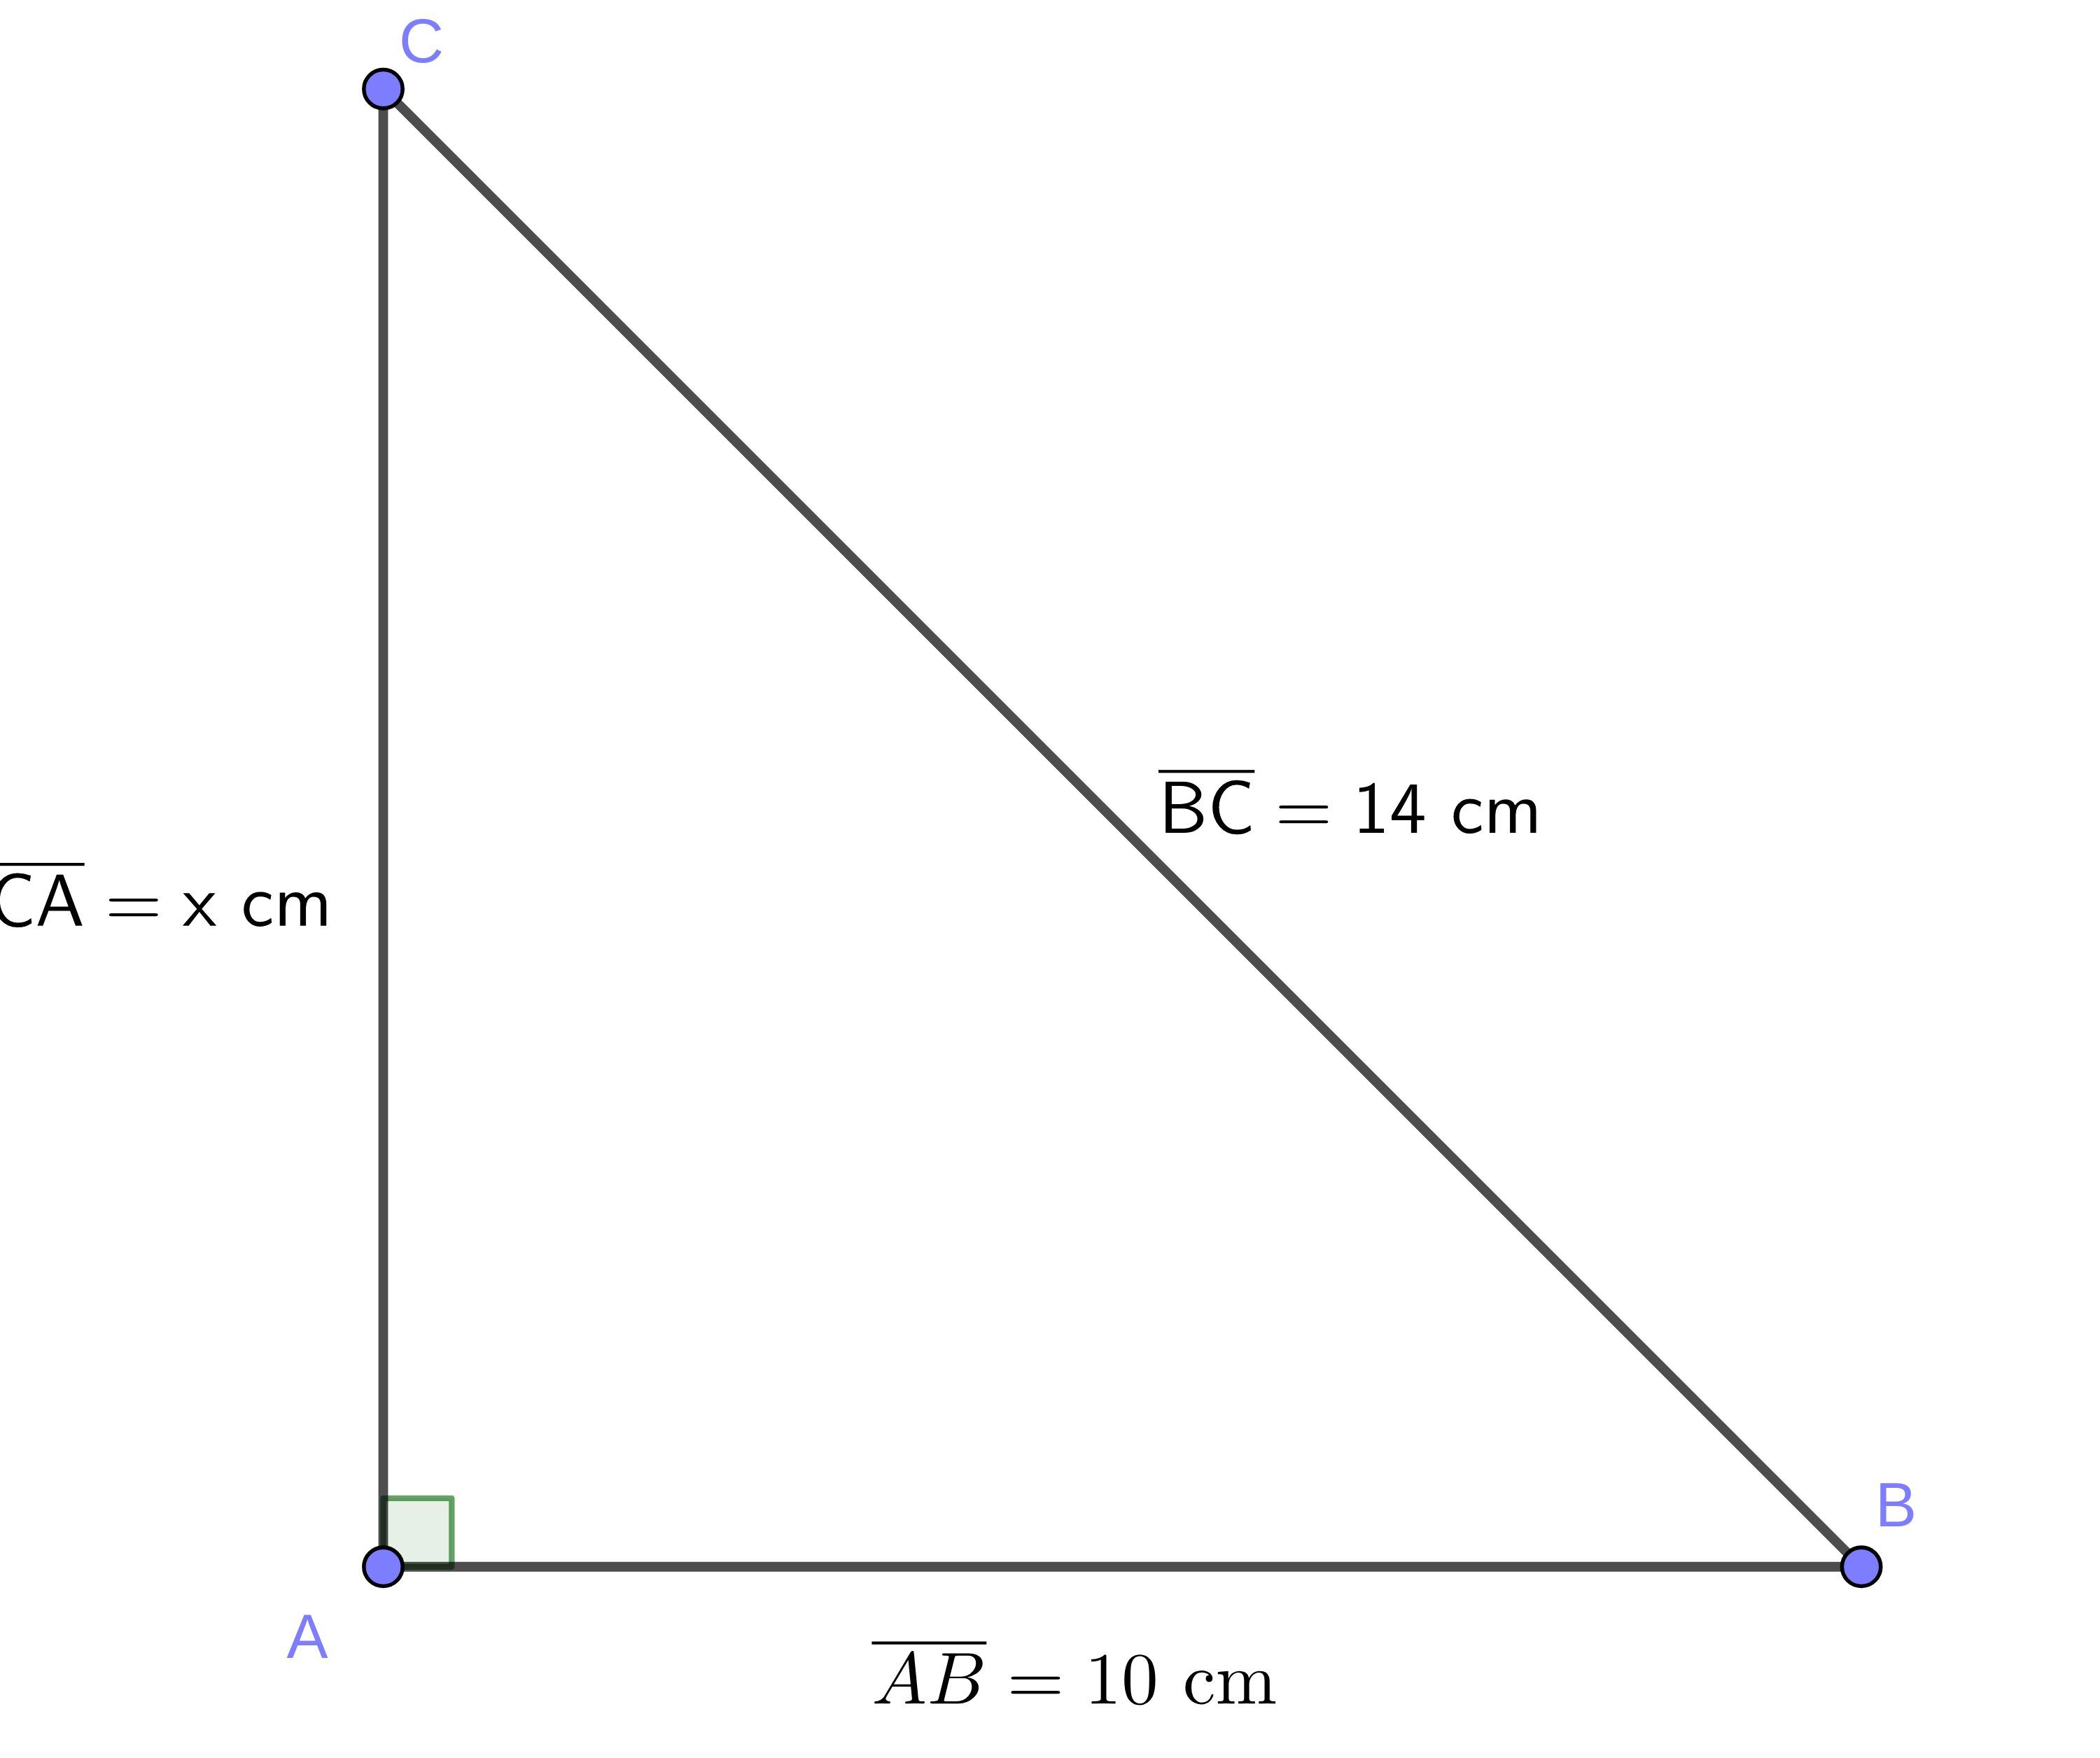
\includegraphics[scale=1]{imagens/exercicio.png}
    \caption{Todos somos gênios}
    \label{figura-genios}
\end{figure}

Aqui vem o texto. Aqui vem o texto. Aqui vem o texto. Aqui vem o texto. 
Aqui vem o texto. Aqui vem o texto. Aqui vem o texto. Aqui vem o texto. 
Aqui vem o texto. Aqui vem o texto. Aqui vem o texto. Aqui vem o texto. 
Aqui vem o texto. Aqui vem o texto. Aqui vem o texto. Aqui vem o texto. 

\begin{table}[htb]
    \centering
    \begin{tabular}{|c|c|}
        teste 1 & teste 2 \\
        teste 1 & teste 2 \\
    \end{tabular}
    \caption{Minha primeira tabela}
    \label{minha-tabela}
\end{table}

Aqui vem o texto. Aqui vem o texto. Aqui vem o texto. Aqui vem o texto. 
Aqui vem o texto. Aqui vem o texto. Aqui vem o texto. Aqui vem o texto. 
Aqui vem o texto. Aqui vem o texto. Aqui vem o texto. Aqui vem o texto. 
Aqui vem o texto. Aqui vem o texto. Aqui vem o texto. Aqui vem o texto. 

\section{Aqui vem o título do Desenvolvimento} 

Aqui vem o texto. Aqui vem o texto. Aqui vem o texto. Aqui vem o texto. 
Aqui vem o texto. Aqui vem o texto. Aqui vem o texto. Aqui vem o texto. 
Aqui vem o texto. Aqui vem o texto. Aqui vem o texto. Aqui vem o texto. 
Aqui vem o texto. Aqui vem o texto. Aqui vem o texto. Aqui vem o texto. 
Aqui vem o texto. Aqui vem o texto. Aqui vem o texto. Aqui vem o texto. 

\begin{table}[htb]
    \centering
    \begin{tabular}{|c|c|}
        teste 1 & teste 2 \\
        teste 1 & teste 2 \\
    \end{tabular}
    \caption{Minha primeira tabela}
    \label{minha-outra-tabela}
\end{table}

\subsection{Aqui vem o título da subseção}

Aqui vem o texto \cite{meuartigo}. Aqui vem o texto. Aqui vem o texto. Aqui vem o texto. 
Aqui vem o texto. Aqui vem o texto. Aqui vem o texto. Aqui vem o texto. 
Aqui vem o texto. Aqui vem o texto. Aqui vem o texto. Aqui vem o texto. 
Aqui vem o texto. Aqui vem o texto. Aqui vem o texto. Aqui vem o texto. 

\begin{figure}[htb]
    \centering
    
\includegraphics[scale=0.2]{imagens/logotipo.jpeg}
    \caption{Logo usado no \LaTeX.} %jeito de colocar o nome Latex estilizado
    \label{figura-leao}
\end{figure}

\subsubsection{Aqui vem o título da subseção da subseção}

Aqui vem o texto. Aqui vem o texto. Aqui vem o texto. Aqui vem o texto. 
Aqui vem o texto. Aqui vem o texto. Aqui vem o texto. Aqui vem o texto. 
Aqui vem o texto. Aqui vem o texto. Aqui vem o texto. Aqui vem o texto. 
Aqui vem o texto. Aqui vem o texto. Aqui vem o texto. Aqui vem o texto. 

\newpage
\bibliographystyle{plain} %define o estilo da referência bibliográfica
\addcontentsline{toc}{section}{Referências} %Inserção das referências no sumário
\bibliography{2018-11-27_referencia.bib} %citar o arquivo onde estão escritas as referências

\end{document}